\chapter{Détection de groupes pertinents dans les flots de liens}
\minitoc
Nous avons vu précédemment qu'il était possible de trouver des groupes de liens dans un flots de liens via l'intermédiaire d'une projection du flot de liens en un graphe statique.
Parmi l'ensemble de ces groupes, il se peut que certains capturent des structures plus importantes et plus pertinentes que d'autres.
Le but ici est de réussir à extraire parmi ces groupes ceux qui sont pertinents.
En ce sens, nous nous posons la question de la décomposition partielle d'un flot de liens en sous-flots pertinents.
Il s'agit donc d'un problème légèrement différent de la détection de partition car certains liens peuvent n'appartenir à aucun groupe et les groupes doivent être pertinents.

Toute la difficulté pour réussir à trouver les groupes pertinents revient à trouver une définition convaincante de la pertinence.
La notion de densité est une première approche mais ce n'est pas suffisant.
En effet comme on a pu le voir précédemment, il peut exister de très grand groupes peu dense et de petits groupes très denses.
Faire la différence entre ces deux catégories en utilisant juste la densité n'est pas possible.
C'est pourquoi, nous utilisons une notion de voisinage.
Un groupe est alors pertinent si il est plus dense que son voisinage.
Ainsi, un groupe peu dense peut être pertinent si il est plus dense que son voisinage.
Comme le but est de pouvoir décrire le flot de liens, nous nous limitons aux groupes ayant une taille supérieur à un minimum.
Un exemple de flots avec une décomposition en groupes pertinent est dans la figure~\ref{fig:exemple_groupe_dens}.

Afin de trouver des des groupes pertinents, nous procédons de la manière suivantes:
\begin{itemize}
\item Nous construisons la projection du flot de liens en un graphe statique;
\item Nous appliquons sur cette projection un algorithme de détection de communautés afin d'obtenir une partition des liens du flot de liens;
\item Nous ne gardons dans la partition que les groupes qui sont considérés comme pertinent, c'est-à-dire ceux qui sont assez gros et qui sont plus dense que leur voisinage.
\end{itemize}

Afin de montrer la pertinence de cette approche, nous l'appliquons sur différents jeux de données et essayons de faire une analyse manuelle de certains groupes trouvés.
Par ailleurs, nous montrons que les groupes que nous détectons ne le sont pas par une méthode statique.

Le chapitre est organisé de la manière suivante.
Dans la section~\ref{sec:groupe_dense_existant}, nous revenons sur les travaux existants qui traitent de sujets similaire.
Puis dans la section~\ref{sec:groupe_dense_method}, nous présentons notre méthode de détection et de validation de groupes pertinents.
Enfin, les jeux de données que nous utilisons sont présentés dans la section~\ref{sec:groupe_dense_result} et les résultats associés dans la section~\ref{sec:groupe_dense_data}.

\begin{figure}
\centering
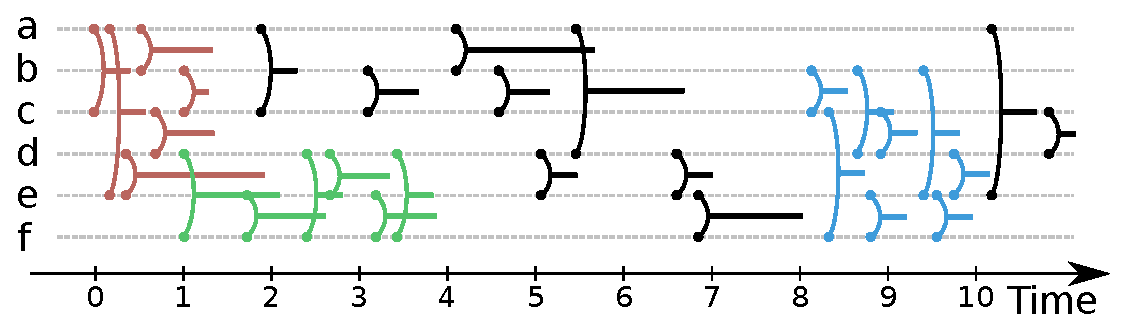
\includegraphics[width=\linewidth]{img/GroupeDense/GroupExample/Zone_dense.eps}
\caption{Exemple de flots de liens avec 3 groupes denses représenté par la couleur des liens (\textcolor{brique}{\textbf{rouge}}, \textcolor{vert_turquoise}{\textbf{vert}} et \textcolor{bleu_window}{\textbf{bleu}}).
}
\label{fig:exemple_groupe_dens}
\end{figure}

\section{Travaux existants}
\label{sec:groupe_dense_existant}

Comme nous l'avons vu dans le chapitre~\ref{chap:etat_art}, il existe assez peu de méthodes cherchant une structure dans un formalisme sans perte d'information.

Mitra~\emph{et al.}~\cite{Mitra2012a} et Speidel~\emph{et al.}~\cite{Speidel2015} ont développé une méthode de détection de communauté mais dans les réseaux diachronique.
Dans un tel réseau, ce sont les n\oe uds qui ont un \emph{timestamp} et non les liens.
Ce cas de figure s'applique parfaitement aux citations car une citation relie bien deux publications qui sont chacune apparues à une date spécifique.
Cependant ce genre de construction est différente n'est pas équivalente au formalisme de flot de liens.
C'est pourquoi nous ne pouvons utiliser la même méthode. 

Ils existent également des méthodes capturant la partie la plus dense du réseau.
C'est le cas de Bogdanov~\emph{et al.}~\cite{Bogdanov2011} qui considèrent encore une autre variante d'extension de graphe.
Ils considèrent un graphe dont la topologie n'évolue pas mais dont le poid des liens change en fonction du temps entre $-1$ et $1$.
Ce formalisme est encore une fois très différent de celui de flot de liens.
De plus, la notion de densité qu'ils utilisent ne tiens pas vraiment compte du temps.
En effet, un groupe de n\oe uds sur intervalle est évalué par la somme des liens entre ces n\oe uds sur tout l'intervalle.


Epasto~\emph{et. al}~\cite{Epasto2015} capture le sous-graphe le plus dense dans un graphe temporel.
Ainsi, le temps est bien pris en compte dans le formalisme.
Cependant, la méthode capture le sous-graphe à un instant $t$ qui est le plus dense.
La notion de densité est donc statique car elle ne considère que la structure de graphe à l'instant $t$.


Enfin il existe les travaux de Rozenshtein~\emph{et. al}~\cite{rozenshtein2014} qui se rapprochent le plus de notre méthode.
Leur méthode considère le formalise de flots de liens et ne suppose pas de structure de graphe à un instant donné.
Elle capture un groupe de n\oe uds et plusieurs intervalles disjoints de telle sorte que ce groupe de n\oe uds dans le graphe agrégé sur ces intervalles ait le degré moyen le plus élevé.
Ainsi même si la méthode permet de capturer un groupe de n\oe uds sur des intervalles, elle évalue un candidat sur le graphe agrégé pour appliquer une métrique de graphe.
Le temps n'a donc pas d'influence sur l'évaluation.
Par ailleurs, leur méthode repose sur plusieurs paramètres qui doivent être fixés \emph{a priori}: le nombre maximum d'intervalle disjoint et la durée cumulée maximum de ces intervalles.
Le premier paramètre permet d'éviter d'utiliser une infinité d'intervalle qui seraient chacun centré sur un lien.
Le second paramètre permet d'éviter de considérer tout le graphe agrégé et ainsi d'obliger la prise en compte du temps.
Ainsi, leur méthode dépend de manière non triviale sur le choix des paramètres.

\bigskip

Pour résumer, il existe des méthodes cherchant la structure la plus dense dans un contexte dynamique; soit en considérant un graphe temporel soit en considérant un flot de liens.
Cependant, ces méthodes utilisent des métriques de graphes pour évaluer un groupe de n\oe uds.
Le temps n'est donc complètement pris en compte dans l'évaluation.
De manière plus importante, ces méthodes évaluent de manière absolue sans prendre en compte de notion de voisinage.
Enfin, nous capturons plusieurs groupes de liens alors qu'ils capturent un groupe n\oe ud.
Certaines des méthodes existantes peuvent être étendues pour capturer les $k$ groupes de n\oe uds les plus denses mais cela se fait au prix de l'ajout d'un paramètre pour contrôler le chevauchement entre deux groupes capturés.


\section{Détection de groupes pertinent}
\label{sec:groupe_dense_method}

Nous avons défini dans le chapitre précédent~\ref{sec:fail_mailing} une transformation du flot de liens en un graphe statique.
Sur cette transformation, nous appliquons un algorithme de détection de communautés.
Nous considérons les communautés trouvées par l'algorithmes comme des groupes potentiellement pertinents.
Nous les appelons donc groupes candidats.

L'ensemble des groupes candidats ne sont pas forcément pertinents.
Tout d'abord, les groupes d'une partition peuvent avoir des tailles très variées.
En particulier, il peut y avoir beaucoup de très petits groupes de $1$ ou $2$ liens.
Ces groupes ne sont pas prise en compte car nous fixons une limite arbitraire sur la taille minimum des groupes.

Par ailleurs, l'algorithme de Louvain optimise de manière gloutonne la modularité dans la transformation du flot de liens en un graphe statique et non une métrique de flot de liens directement.
C'est pourquoi, certains candidats peuvent être une bonne communauté dans le graphe mais un groupe non pertinent dans le flot de liens.
Cet effet est d'autant plus présent que la modularité ne prend pas en compte le voisinage d'un groupe.
Par exemple dans la figure~\ref{fig:exemple_groupe_dens}, les liens dans l'intervalle $[4,8]$ forment une composante connexe dans la transformation et ils sont considérés comme une communauté par l'algorithme de Louvain.
Or, ce candidat n'est pas un groupe pertinent car il est beaucoup moins dense que les liens durant l'intervalle $[0,4]$ ou l'intervalle $[7,11]$.
C'est pourquoi il est nécessaire de valider ou de filtrer les groupes candidats pour ne garder que les groupes pertinents.




\subsection{Définition du voisinage}
Dans le chapitre~\ref{sec:def_densite}, nous avons défini la densité d'un flot de liens.
Pour la densité d'un groupe de liens, il faut donc calculer la densité du sous flots induit par ces liens.
Il est donc possible de calculer la densité d'un candidat.
Seulement, la densité en elle même n'est pas un bon critère pour évaluer la pertinence d'un candidat.
En effet, un candidat constitué d'un unique lien a une densité de maximal de $1$.
C'est pourquoi il est également nécessaire de tenir compte du voisinage.
Ainsi, plus le candidat a une densité plus importante que son voisinage, plus le candidat est un groupe pertinent.

Il est donc nécessaire de définir une notion de voisinage qui puisse tenir compte à la fois de la structure et du temps.
Pour ce faire, il faut utiliser une autre définition de la densité pour comprendre quels sont les paramètres qui influent sur la densité.
Jusqu'à maintenant pour un candidat $C_i$, nous considérons la densité du sous flot induit par ses liens,$\delta(L(C_i))$.
Pour faire apparaitre l'influence de la structure et du temps, nous utilisons $\delta(L_{\beta(C_i)..\psi(C_i)}(V(C_i)^2))$ que nous simplifions par $\delta(V(C_i),\beta(C_i), \bar{C_i})$ où $\bar{C_i} = \psi(C_i)-\beta(C_i)$.
Il s'agit de la densité des n\oe uds induits par $C_i$ sur la durée du groupe.
Ces deux formulations ne sont pas équivalentes car les deux sous flots ne sont pas équivalent en particulier $L(C_i) \subseteq L_{\beta(C_i)..\psi(C_i)}(V(C_i)^2)$.
De cette inclusion découle le fait $\delta(L(C_i)) \leq \delta(V(C_i),\beta(C_i), \bar{C_i})$.
C'est le cas dans l'exemple de la figure~\ref{fig:exemple_groupe_dens} si l'on veut calculer la densité des liens noirs.
Dans ce cas, l'ensemble de n\oe uds induit par ces liens est égale à $V$ et l'intervalle de temps est égale à $[2,11]$.
Le sous flot induit par $V$ sur $[2,11]$ comprend l'ensemble des liens noirs mais aussi des liens \textcolor{vert_turquoise}{\textbf{verts}} et \textcolor{bleu_window}{\textbf{bleus}}.


Cependant avec cette formulation, on fait apparaitre 3 dimensions: l'ensemble de n\oe uds, le temps de début et la durée.
Il devient alors aisé de considérer comme voisins les sous flots qui différent sur une seule dimension: soit le temps de début, soit la durée soit les n\oe uds.
Cette différence entre les voisinages est illustrée dans la figure~\ref{fig:voisinage_groupe}.

\begin{figure}
\centering
	\begin{subfigure}{0.3\textwidth}
		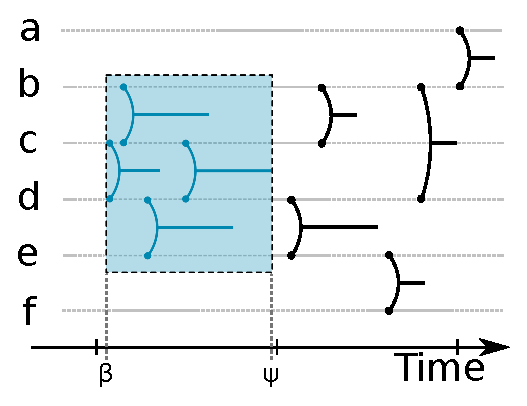
\includegraphics[height=3cm]{img/GroupeDense/GroupExample/Voisinage/Base.eps}
		\caption{Groupe de liens initial}
	\end{subfigure}\hspace*{0.05cm}

	\begin{subfigure}{0.3\textwidth}
		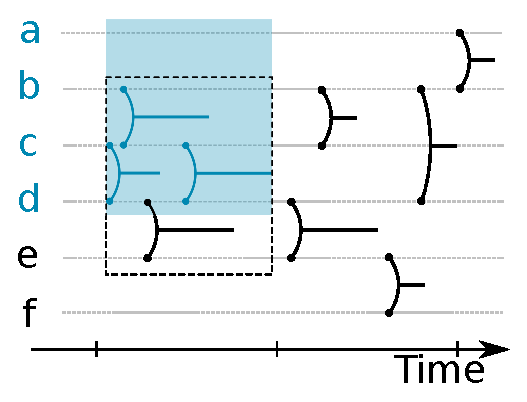
\includegraphics[height=3cm]{img/GroupeDense/GroupExample/Voisinage/Variable_Nodes.eps}
		\caption{Voisinage sur les n\oe uds}
	\end{subfigure}\hspace*{0.05cm}
	\begin{subfigure}{0.3\textwidth}
		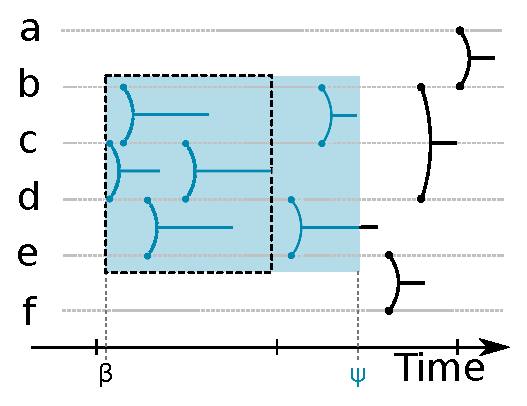
\includegraphics[height=3cm]{img/GroupeDense/GroupExample/Voisinage/Variable_duration.eps}
		\caption{Voisinage sur la durée}
	\end{subfigure}\hspace*{0.05cm}
	\begin{subfigure}{0.3\textwidth}
		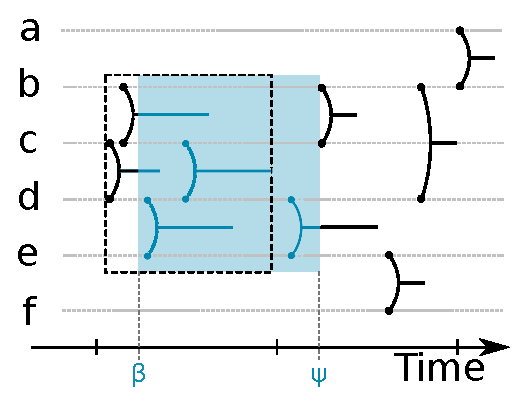
\includegraphics[height=3cm]{img/GroupeDense/GroupExample/Voisinage/Variable_start.eps}
		\caption{Voisinage sur le temps de début}
	\end{subfigure}	
	\caption{Exemple d'un groupe de liens en (A) et de ses différents voisinage en (B), (C) et (D).
	La zone en \textcolor{bleu_transparent}{\textbf{bleu}} est la zone prise en compte lors du calcul de la densité.
	La zone en pointillé représente la zone considérée lors du calcul de la densité du groupe initial.
	}
	\label{fig:voisinage_groupe}
\end{figure}


Pour le voisinage au n\oe uds, il est impossible de considérer l'ensemble de tous les ensemble de n\oe uds car il est beaucoup trop grand.
De plus, il est probable que ces groupes de n\oe uds ne soient pas connectés si le flot de liens est peu dense.
C'est pourquoi, si $V(C_i)$ contient $k$ n\oe uds, nous nous limitons à l'ensemble des groupes de $k$ n\oe uds qui partage $k-1$ n\oe uds avec $V(C_i)$.
De cette manière, uniquement des groupes de n\oe uds similaires au candidat sont considérés.
Cette comparaison nous semble plus stricte mais plus équitable que celles utilisant l'ensemble des groupes de n\oe uds ou des groupes de n\oe uds pris aléatoirement.
Il serait possible de considérer un nombre moins important de n\oe uds partagés mais nous ne l'avons pas fait à cause de la complexité de calcul.
En effet, partager $k-1$ n\oe uds entraine la création $k(|V|-k)$ sous flots pour le voisinage au n\oe uds pour un unique candidat.

Pour le voisinage au temps de début(resp. à la durée), nous considérons toutes les valeurs possibles de temps début (resp. durée) dans un intervalle donné.
Chacune de ces valeurs donne lieu à un sous flot induit ayant les mêmes n\oe uds et la même durée (resp. temps de début) que le sous flot du groupe candidat.
Ensuite, nous calculons la densité de chacun de ces sous flots voisins.
Pus formellement, l'ensemble des densités des sous flots voisin se défini de la manière suivante.
Soit $I_1$ et $I_2$ deux intervalles et $C_i$ un groupe de liens.
Les densités des sous flot dans le voisinage au temps de début sont alors définies par la fonction $\delta(V(C_i),x, \bar{C_i})$, $\forall x \in I_1$.
Les densités des sous flot dans le voisinage de la durée sont alors définies par la fonction $\delta(V(C_i),\beta(C_i), y)$, $\forall y \in I_2$.

L'intervalle utilisé pour le voisinage au temps de début $[\alpha, \omega-\bar{C_i}]$.
Pour le voisinage à la durée, nous utilisons l'intervalle $[0.8\Delta_{min}, 1.2\Delta_{max}]$, où $\Delta_{min}$ (resp. $\Delta_{max}$) est la plus petite (resp. grande) durée de tous les candidats considérés initialement.
Nous utilisons cet intervalle pour deux raisons.
Tout d'abord, il contient l'ensemble des durée acceptables quand nous l'appliquons à nos jeux de données.
Mais surtout, nous avons également testé l'intervalle $[1-\omega-\alpha]$ qui est beaucoup plus grand.
Cela change les résultat de manière quantitative mais pas de manière qualitative.
En effet lorsque la durée considérée est proche de $\omega-\alpha$ alors la densité est très proche de $0$.
Comme ces valeurs sont peu informative, nous préférons nous limiter à un intervalle un peu plus restreint.
\bigskip

Au final, nous avons pour chaque voisinage les valeurs de densités des sous flots voisins.
Pour le voisinage au n\oe uds, il y a $k(|V|-k)$ valeurs de densité différentes.
Pour le voisinage au temps de début(resp. à la durée), nous avons une fonction de la densité qui dépend du temps de début (resp. de la durée).


\subsection{Définition de l'évaluation}
Nous évaluons chaque candidat en comparant sa densité à celle des sous flots dans chaque voisinage.
Si un candidat est vraiment pertinent alors il devrait avoir une densité significativement plus élevée que la plupart des sous flots voisins.
Si la densité des sous flots voisins suivait une distribution connue, par exemple une loi normale, alors cela reviendrait à évaluer si la densité du candidat est éloignée de la moyenne en observant le \emph{z-score}.
De par nos observations, les distributions de densités des sous flots voisins ne suivent pas la même distribution pour différent candidats.
Par exemple dans la figure~\ref{fig:distrib_dens}, des distributions cumulatives de la densité pour le voisinage à la durée pour 3 groupes candidats des jeux de donnée Socio pattern et Rollernet\,\footnote{Ces jeux de données sont présenté dans la section suivante~\ref{sec:groupe_dense_data}.} sont présentées.
Ces distributions sont très différentes et il n'est pas donc pas justifié d'assumer une unique distribution sous-jacente.
C'est pourquoi nous utilisons les \emph{percentiles} qui représentent la proportion des valeurs de densités qui sont inférieures à la densité du candidat.


\begin{figure}
\centering
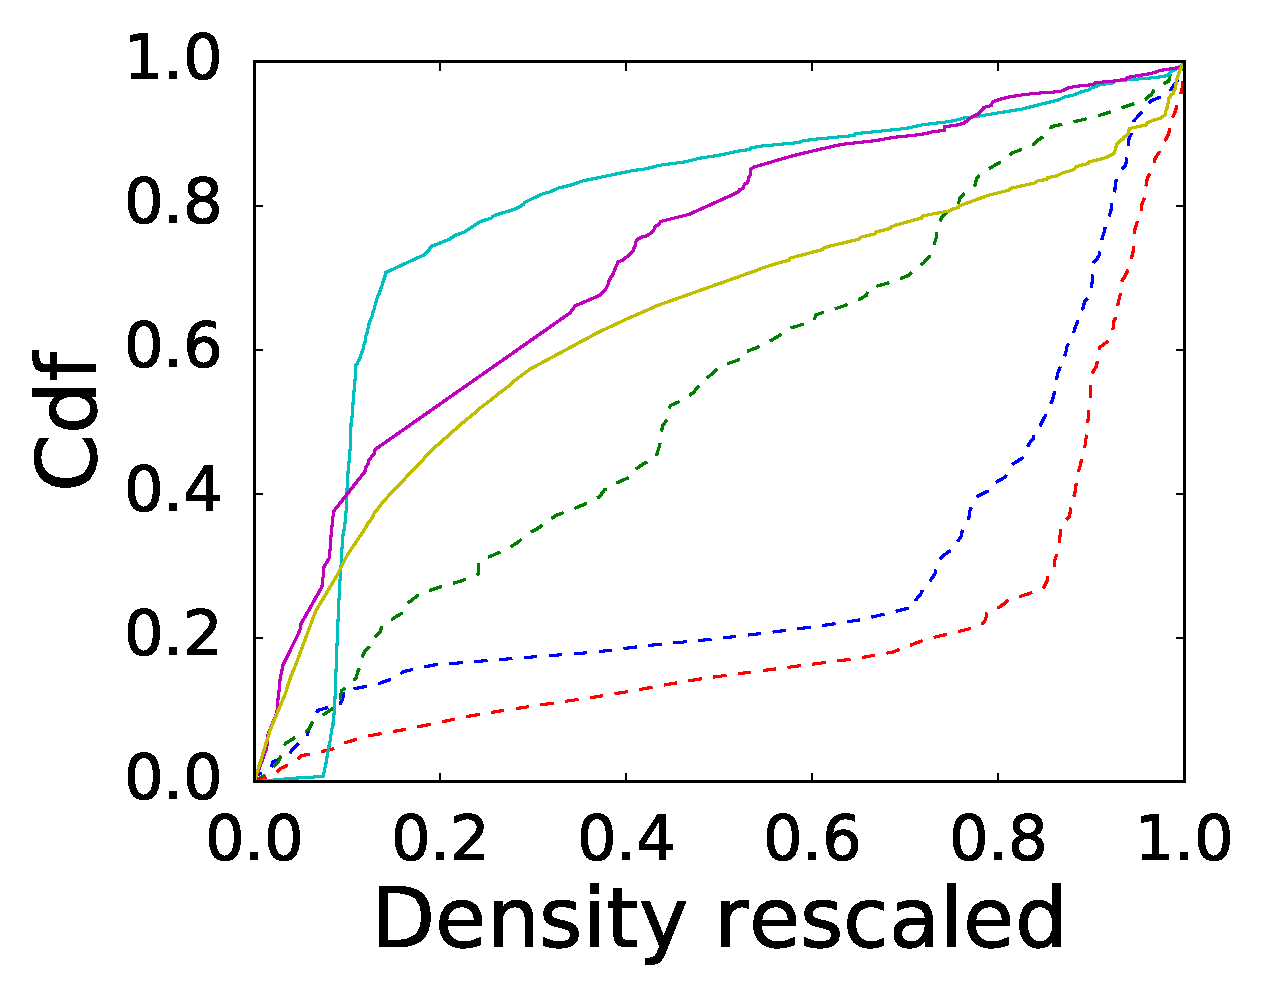
\includegraphics[width=0.3\linewidth]{img/GroupeDense/cdf_density_duration.eps}
\caption{Distribution cumulative (\emph{cdf}) des valeurs de densité renormalisées  des sous flots voisins dans le voisinages à la durée.
En train plein (resp. pointillé), candidats du jeux de données Rollernet (resp. Socio pattern).}
\label{fig:distrib_dens}
\end{figure}

Pour le voisinage au n\oe uds qui est représenté par un ensemble, $S$, de valeurs de densité, le score d'un candidat $C_i$ ayant une densité, $\delta^*$, est:

\begin{equation}
p_{noeud}(C_i)= \dfrac{\sum_{\delta \in S} \mathbf{1}_{\delta \le \delta^*}}{|S|}\,,
\end{equation}
où $\mathbf{1}$ est la fonction indicatrice.
Pour le voisinage au temps de début et à la durée qui sont représentés par des fonctions, les scores sont respectivement:

\begin{equation}
p_{d\acute{e}but}(C_i)=\dfrac{1}{\omega-\bar{C_i} - \alpha} \int_{\alpha}^{\omega- \bar{C_i}} \mathbf{1}_{\delta(V(C_i),z,\bar{C_i}) <\delta^*} dz \ ,
\end{equation} 
\begin{equation}
p_{dur\acute{e}e}(C_i)=\dfrac{1}{1.2\Delta_{max} - 0.8\Delta_{min}} \int_{0.8\Delta_{min}}^{1.2\Delta_{max}} \mathbf{1}_{\delta(V(C_i),\beta(C_i),z) <\delta^*} dz \, .
\end{equation}

Un score de $15\%$ pour un type de voisinage signifie que la densité du candidat est plus faible que $85\%$ des sous flots voisins de ce type et que par conséquent le candidat ne devrait pas être considéré comme pertinent.

\bigskip
Pour résumer, un candidat est évalué par un triplet constitué des scores obtenus pour chaque voisinage.
Un candidat est considéré comme pertinent si tous ces scores sont plus élevés que des seuils définis manuellement.
La définition de ces seuils est difficile et dépend des caractéristiques du flot de liens.
C'est pourquoi nous ne les fixons pas \emph{a priori} mais \emph{a posteriori} après avoir examiner la distribution des scores.
Le choix des seuil est décris plus amplement dans la section~\ref{sec:groupe_dense_result}.


\section{Jeux de données}
\label{sec:groupe_dense_data}
Nous appliquons notre méthodes sur 4 jeux de données différents.
La table~\ref{tab:data_spec_groupe_dense} listent le nombre de n\oe uds, le nombre de liens et la durée de chaque jeu de données.

\begin{table}
\centering
% table caption is above the table

% For LaTeX tables use
\begin{tabular}{|c|c|c|c|}
\hline  \rule[-1ex]{0pt}{3.5ex}
Datasets & $|V|$ & $|E|$ & $\omega - \alpha$  \\
\hline
Socio pattern & 180 & 19774 & 9 jours \\
Rollernet & 62 & 15803 &  3 heures\\
Reality Mining & 94 & 44975 & 9 mois\\
Babouins & 28 & 95616 & 14 jours\\
\hline
\end{tabular}
\caption{nombre de n\oe uds $|V|$,nombre de liens $|E|$ et durée de chaque jeu de données.}
\label{tab:data_spec_groupe_dense} 
\end{table}

\begin{description}
\item[Socio Pattern~\cite{Fournet2014}\,\footnote{\url{http://www.sociopatterns.org}}] contient le réseaux dynamique d'étudiant d'une classe préparatoire à Marseilles en 2012. $180$ étudiants de $5$ classes ont porté pendant $9$ jours des capteurs de proximités.
Ainsi, il est possible de savoir quand $2$ interagissent. 
Dans ce jeu de de donnée, la classe de chaque étudiant est connue.\\

\item[Rollernet~\cite{Tournoux2009}] a été collecté durant une randonné roller ayant eu lieu en 2066.
Il s'agit d'un ayant regroupé $2500$ participants.
Parmi eux, $62$ étaient équipé d'appareils \emph{bluetooth} qui enregistrent l'ensemble des appareils \emph{bluetooth} disponibles.
Nous nous limitons uniquement aux contacts ayant eu lieu entre les $62$ personnes portant un capteur.
Des métadonnées sont également associés et notamment le rôle de chaque personne.
Un rôle peut être membre de l'organisation à l'avant du peloton ou membre d'une association de roller.\\

\item[Reality Mining~\cite{Eagle2009}] représente le réseau d'interactions entre $94$ personnes du \emph{MIT Media Laboratory} entre Septembre 2004 et Juin 2005.
Parmi les $94$ participants, $68$ évoluent dans le même bâtiment (90\% étudiants, 10\% employés) alors que le reste sont des étudiants de l'école de commerce de l'université.
Ce jeu de donné a été récolté grâce à des téléphones \emph{bluetooth} prêtés aux étudiants.\\

\item[Babouins~\cite{Crofoot2015,Strandburg-Peshkin2015}] contient la position \emph{GPS} de $28$ babouins (\emph{Papio anubis}) dans le centre de recherche Mpala au Kenya.
Ces $28$ babouins représentent $80\%$ d'une troupe.
Chaque babouin est équipé d'un collier muni d'un capteur \emph{GPS} qui enregistre la position toute les secondes.
Nous transformons ces données en un flot de liens en créant un lien de entre deux babouins si ils sont à moins de 1 mètre 50 durant les dernières 10 secondes pour lisser les potentielles imprécisions du \emph{GPS}.
Le code est disponible en ligne\,\footnote{https://bitbucket.org/nGaumont/baboonstreamextractor} et est écris en \emph{rust}.
\end{description}

Même si ces jeux de données sont des réseaux d'interactions face-à-face, ils sont différents dans leur dynamique.
Par exemple, le jeu de donnée Rollernet a environ le même nombre de liens que celui de Socio Pattern alors qu'il dure seulement 3 heures contre 9 jours pour Socio Pattern.
Enfin, nous n'incluons pas le jeu de données de courriels utilisé précédemment car notre méthode nécessite un flot de liens avec durées.
Nous pourrions utilisés un flot de liens avec une durée artificiellement mais le choix de la durée impacte les scores.



\section{Application}
\label{sec:groupe_dense_result}

Pour chaque jeu de données, nous appliquons notre méthode pour capturer les groupes d'interactions pertinents.
Comme présenté dans la section~\ref{sec:groupe_dense_method}, la première étape est de trouver une partition, $\mathcal{C}$, des liens.
Quelques statistiques obtenues pour chaque partition sont listées dans la table~\ref{tab:partition_spec_gd}, notamment les nombres de n\oe uds et de liens médians.
La première chose qui est frappante est qu'il existe énormément de très petits groupes.
On remarque également que seul le jeu de données Rollernet se distingue des autres en ayant des groupes plus gros.
Cette différence est probablement due au flot de liens qui contient beaucoup de liens pour uniquement 3 heures de durée.
Afin d'avoir une vision plus précise pour le jeu de données Socio Pattern, nous présentons dans la figure~\ref{fig:distri_group_SP} les distributions cumulatives inverses du nombre de n\oe uds, du nombre de liens, de la durée et de la densité des groupes.


\groupcharac{Sociopattern}{Socio Pattern}{SP}

%\groupcharac{RollernetLim}{Rollernet}{rollernet}
%\groupsPerNode{RollernetLim}{Rollernet}{rollernet}
%\percentile{RollernetLim}{Rollernet}{rollernet}
%\groupcharacFilter{RollernetLim}{Rollernet}{rollernet}

\begin{table}
\centering
% table caption is above the table

% For LaTeX tables use
\begin{tabular}{|c|c|c|c|}
\hline \rule[-1ex]{0pt}{3.5ex}
Datasets & $|\mathcal{C}|$ & $\langle|V|\rangle$  & $\langle|L|\rangle$ \\
\hline
Socio Pattern & 12532 (155) & 2 (9) & 1 (15) \\
Rollernet& 559 (75) & 2 (31) & 1 (194) \\
Reality Mining & 5737 (474) & 2 (12) & 1 (36) \\
Babouin & 37671 (1249)  &  2 (7)  & 1 (16) \\
\hline
\end{tabular}
\caption{$|\mathcal{C}$|: nombre de groupes dans la partition, $\langle|V|\rangle$ médiane du nombre de n\oe uds dans un groupe, $\langle|L|\rangle$ médiane du nombre de liens dans un groupe.
Les valeurs en parenthèses correspondent à la valeur quand uniquement les groupes d'au moins $10$ liens sont pris en compte.}
\label{tab:partition_spec_gd}       % Give a unique label
\end{table}




\begin{table}
\centering
% table caption is above the table

% For LaTeX tables use
\begin{tabular}{|c|c|c|c|c|c|}
\hline \rule[-1ex]{0pt}{3.5ex}
Datasets & $p_{node}$ & $p_t$  & $p_\delta$ & $N_c$  & execution \\
\hline
Socio Pattern & 0.98 & 0.998 & 0.85 & 136 & 2 min \\
Rollernet& 0.9 & 0.7 & 0.6 & 37 & 4 min \\
Reality Mining & 0.97  & 0.98 & 0.8 & 394 & 1h \\
Babouin & 0.95  &  0.99  & 0.85 & 1023 & 52 min\\
\hline
\end{tabular}
\caption{Threshold used, number of groups captured and execution time for each dataset. $p_{node}$,$p_t$,$p_\delta$ and $N_c$ are respectively the node aspect threshold, the start time aspect threshold, the duration aspect threshold and the number of group captured.}
\label{tab:thresholds}       % Give a unique label
\end{table}


\begin{table*}[t]
\centering
\begin{tabular}{|c|c|c|c|c|c|c|}
\hline  \rule[-1ex]{0pt}{3.5ex}  & $\lambda= 0.05$ &$\lambda= 0.1$ & $\lambda=0.2$ & $\lambda=0.3$ & $\lambda=0.5$ & $\lambda=0.7$ \\ 
\hline Socio pattern & 0.30 (0.55)  & 0.30 (0.55)  & 0.30 (0.55)  & 0.30 (0.55)  & 0.29 (0.54) & 0.33 (\textbf{0.85})  \\ 
\hline Rollernet & 0.40 (0.52) & 0.39 (0.64) & 0.41 (0.54) & 0.37 (0.54) & 0.31 (0.57)  &  0.26 (0.75) \\ 
\hline Reality Mining & 0.42 (0.76)  & 0.42 (0.77) & 0.36 (\textbf{0.88}) & 0.42 (\textbf{0.86}) & 0.38 (\textbf{0.87})  & 0.36 (\textbf{1}) \\ 
\hline Baboons & 0.33 (\textbf{0.95}) & 0.38 (\textbf{1}) & 0.40 (\textbf{0.84}) & 0.46 (\textbf{0.94}) & 0.46 (\textbf{0.93}) & 0.44 (\textbf{0.85}) \\ 
\hline 
\end{tabular} 
\caption{Median (and maximum) Jaccard index between the groups uncovered and the communities found by bigclam in the aggregated graph where  a proportion of $\lambda$ edges having the smallest weight have been removed.
Values which are above $0.8$ are in bold.}
\label{tab:Jaccard}  
\end{table*}
\section{Conclusion et perspective}


\subsection{Jeux de test ?}